\chapter{Architectural aspects of Instant Messaging System}\label{ch:secure-ims-implementation}


\section{Application architecture and UML modeling}\label{sec:application-architecture-and-uml-modeling}

\subsection{Motivation}\label{subsec:motivation}
As a programmers, I believe all we have faced the cases of crucial over-engineering during the implementation of some software product.
For the programmer, it is a vital point to follow two separated, but closely related software development principles, such that
KISS (Keep It Simple and Stupid), and YAGNI (You Aren't Gonna Need It).
As the main topic of our thesis is the security and privacy aspects of Instant Messaging Systems, we consider following
previously discussed principles KISS and YAGNI and use a well-known Monolithic architecture.
One would suggest to use nowadays popular Microservice Architecture, thinking about scalability,
an ability of the system to handle large numbers of users distributed over geographically large areas without notably affecting
the overall performance of the system.
However, the effect of Microservices is felt only for quite large and complex systems, not the case of Instant Messaging System
we implement in chapter [number].
It is worthless to divide the functional requirements, discussed in section [number] into microservices and that's central point
in motivation to use Monolithic Architecture.
Following plot demonstrates the relation between complexity of system and architecture.

\begin{figure}[H]
    \centering
    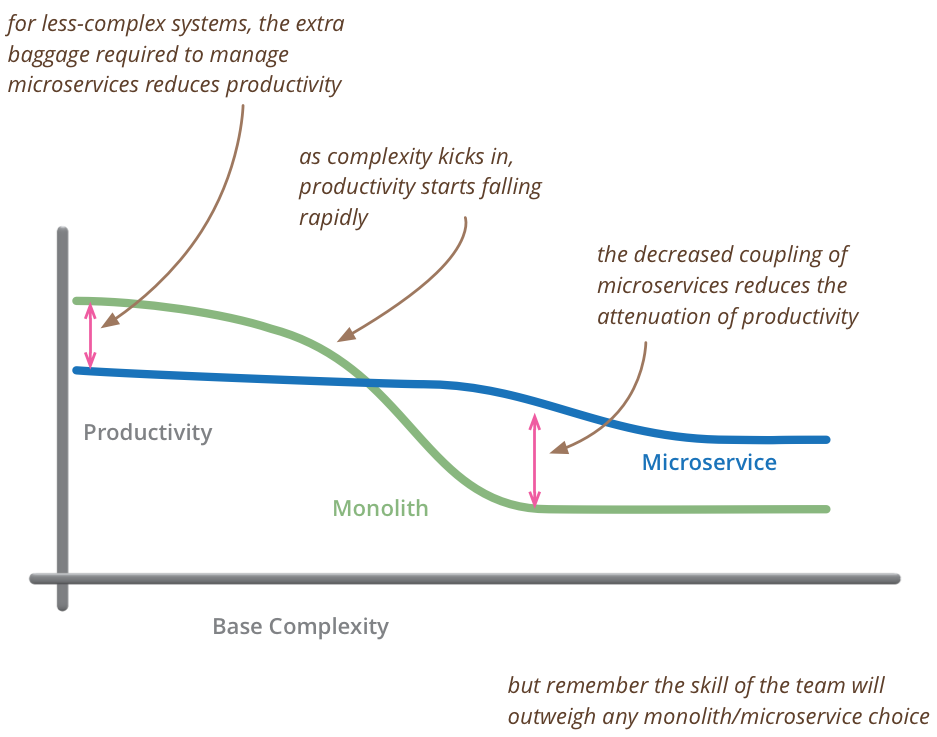
\includegraphics[width=1\textwidth]{Pictures/monolith_vs_microservice}
    \caption{Relation between system complexity and architectures. Source: https://martinfowler.com/bliki/MicroservicePremium.html}
    \label{fig:monolith_vs_microservice}
\end{figure}

\subsection{Initial concept diagram and discussion}\label{subsec:initial-concept-diagram}
\begin{figure}[H]
    \centering
    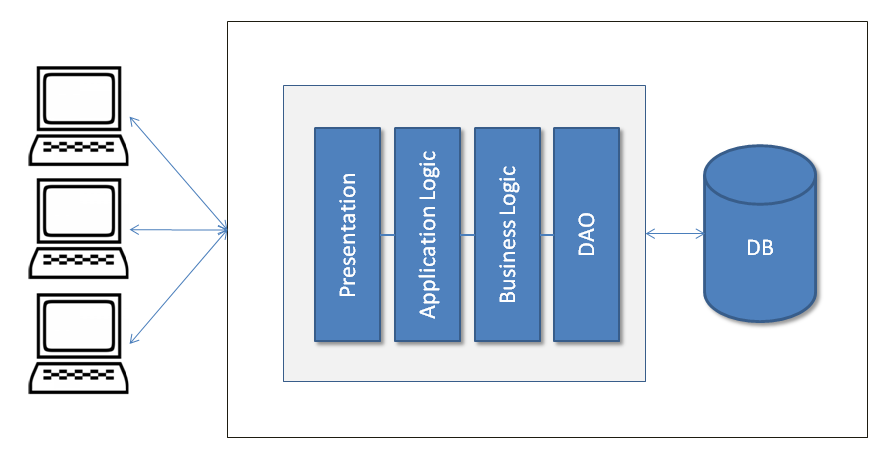
\includegraphics[width=1\textwidth]{Pictures/monolith_architecture}
    \caption{Monolithic architecture diagram. Source: }\label{fig:figure2}
\end{figure}

\subsection{Application layers}\label{subsec:application-layers}
\begin{itemize}
    \item Presentation
    \item Application Logic
    \item Business Logic
    \item Data Access Object (DAO)
    \item Database (DB)
\end{itemize}

\subsection{Monolith Architecture: Cons and Props}\label{subsec:monolith-architecture:-cons-and-props}

A monolith is built as a large system with a single code base and deployed as a single unit, usually behind a load balancer.
It typically consists of four major components: a user interface, business logic, a data interface and a database.
Monoliths offer several advantages, particularly when it comes to operational overhead requirements.
Here are some of those basic benefits:

\begin{itemize}
    \item \textbf{Simplicity.} Monolithic architectures are simple to build, test and deploy.
    These apps can scale horizontally, in one direction, by running several copies of the application behind a load balancer.
    Cross-cutting concerns: With a single codebase, monolithic apps can easily handle cross-cutting concerns, such as logging,
    configuration management and performance monitoring.
    Another advantage associated with the simplicity of monolithic apps is easier deployment.
    When it comes to monolithic applications, you do not have to handle many deployments – just one file or directory.
    \item \textbf{Performance.} Components in a monolith typically share memory which is faster than service-to-service communications using
    IPC or other mechanisms.
    \item \textbf{Easier debugging and testing.}
    In contrast to the microservices architecture, monolithic applications are much easier to debug and test.
    Since a monolithic app is a single indivisible unit, you can run end-to-end testing much faster.
    \item \textbf{Easier development.} As long as the monolithic approach is a standard way of building applications,
    any engineering team has the right knowledge and capabilities to develop a monolithic application.
\end{itemize}
But one major drawback of monolithic architectures is tight coupling.
Over time, monolithic components become tightly coupled and entangled.
This coupling effects management, scalability and continuous deployment.
Other cons that stem from tight coupling include:

\begin{itemize}
    \item \textbf{Understanding.} When a monolithic application scales up, it becomes too complicated to understand.
    Also, a complex system of code within one application is hard to manage.
    \item \textbf{Reliability.} An error in any of the modules in the application can bring the entire application down.
    \item \textbf{Updates.} Due to a single large codebase and tight coupling, the entire application would have to deploy
    for each update.
    \item \textbf{Technology stack.} A monolithic application must use the same technology stack throughout.
    Changes to the technology stack are expensive, both in terms of the time and cost involved.
    \item \textbf{Scalability.} You cannot scale components independently, only the whole application.
\end{itemize}

\subsection{Decoupling Monolith using CQRS}\label{subsec:decoupling-monolith-using-cqrs}
\begin{figure}[H]
    \centering
    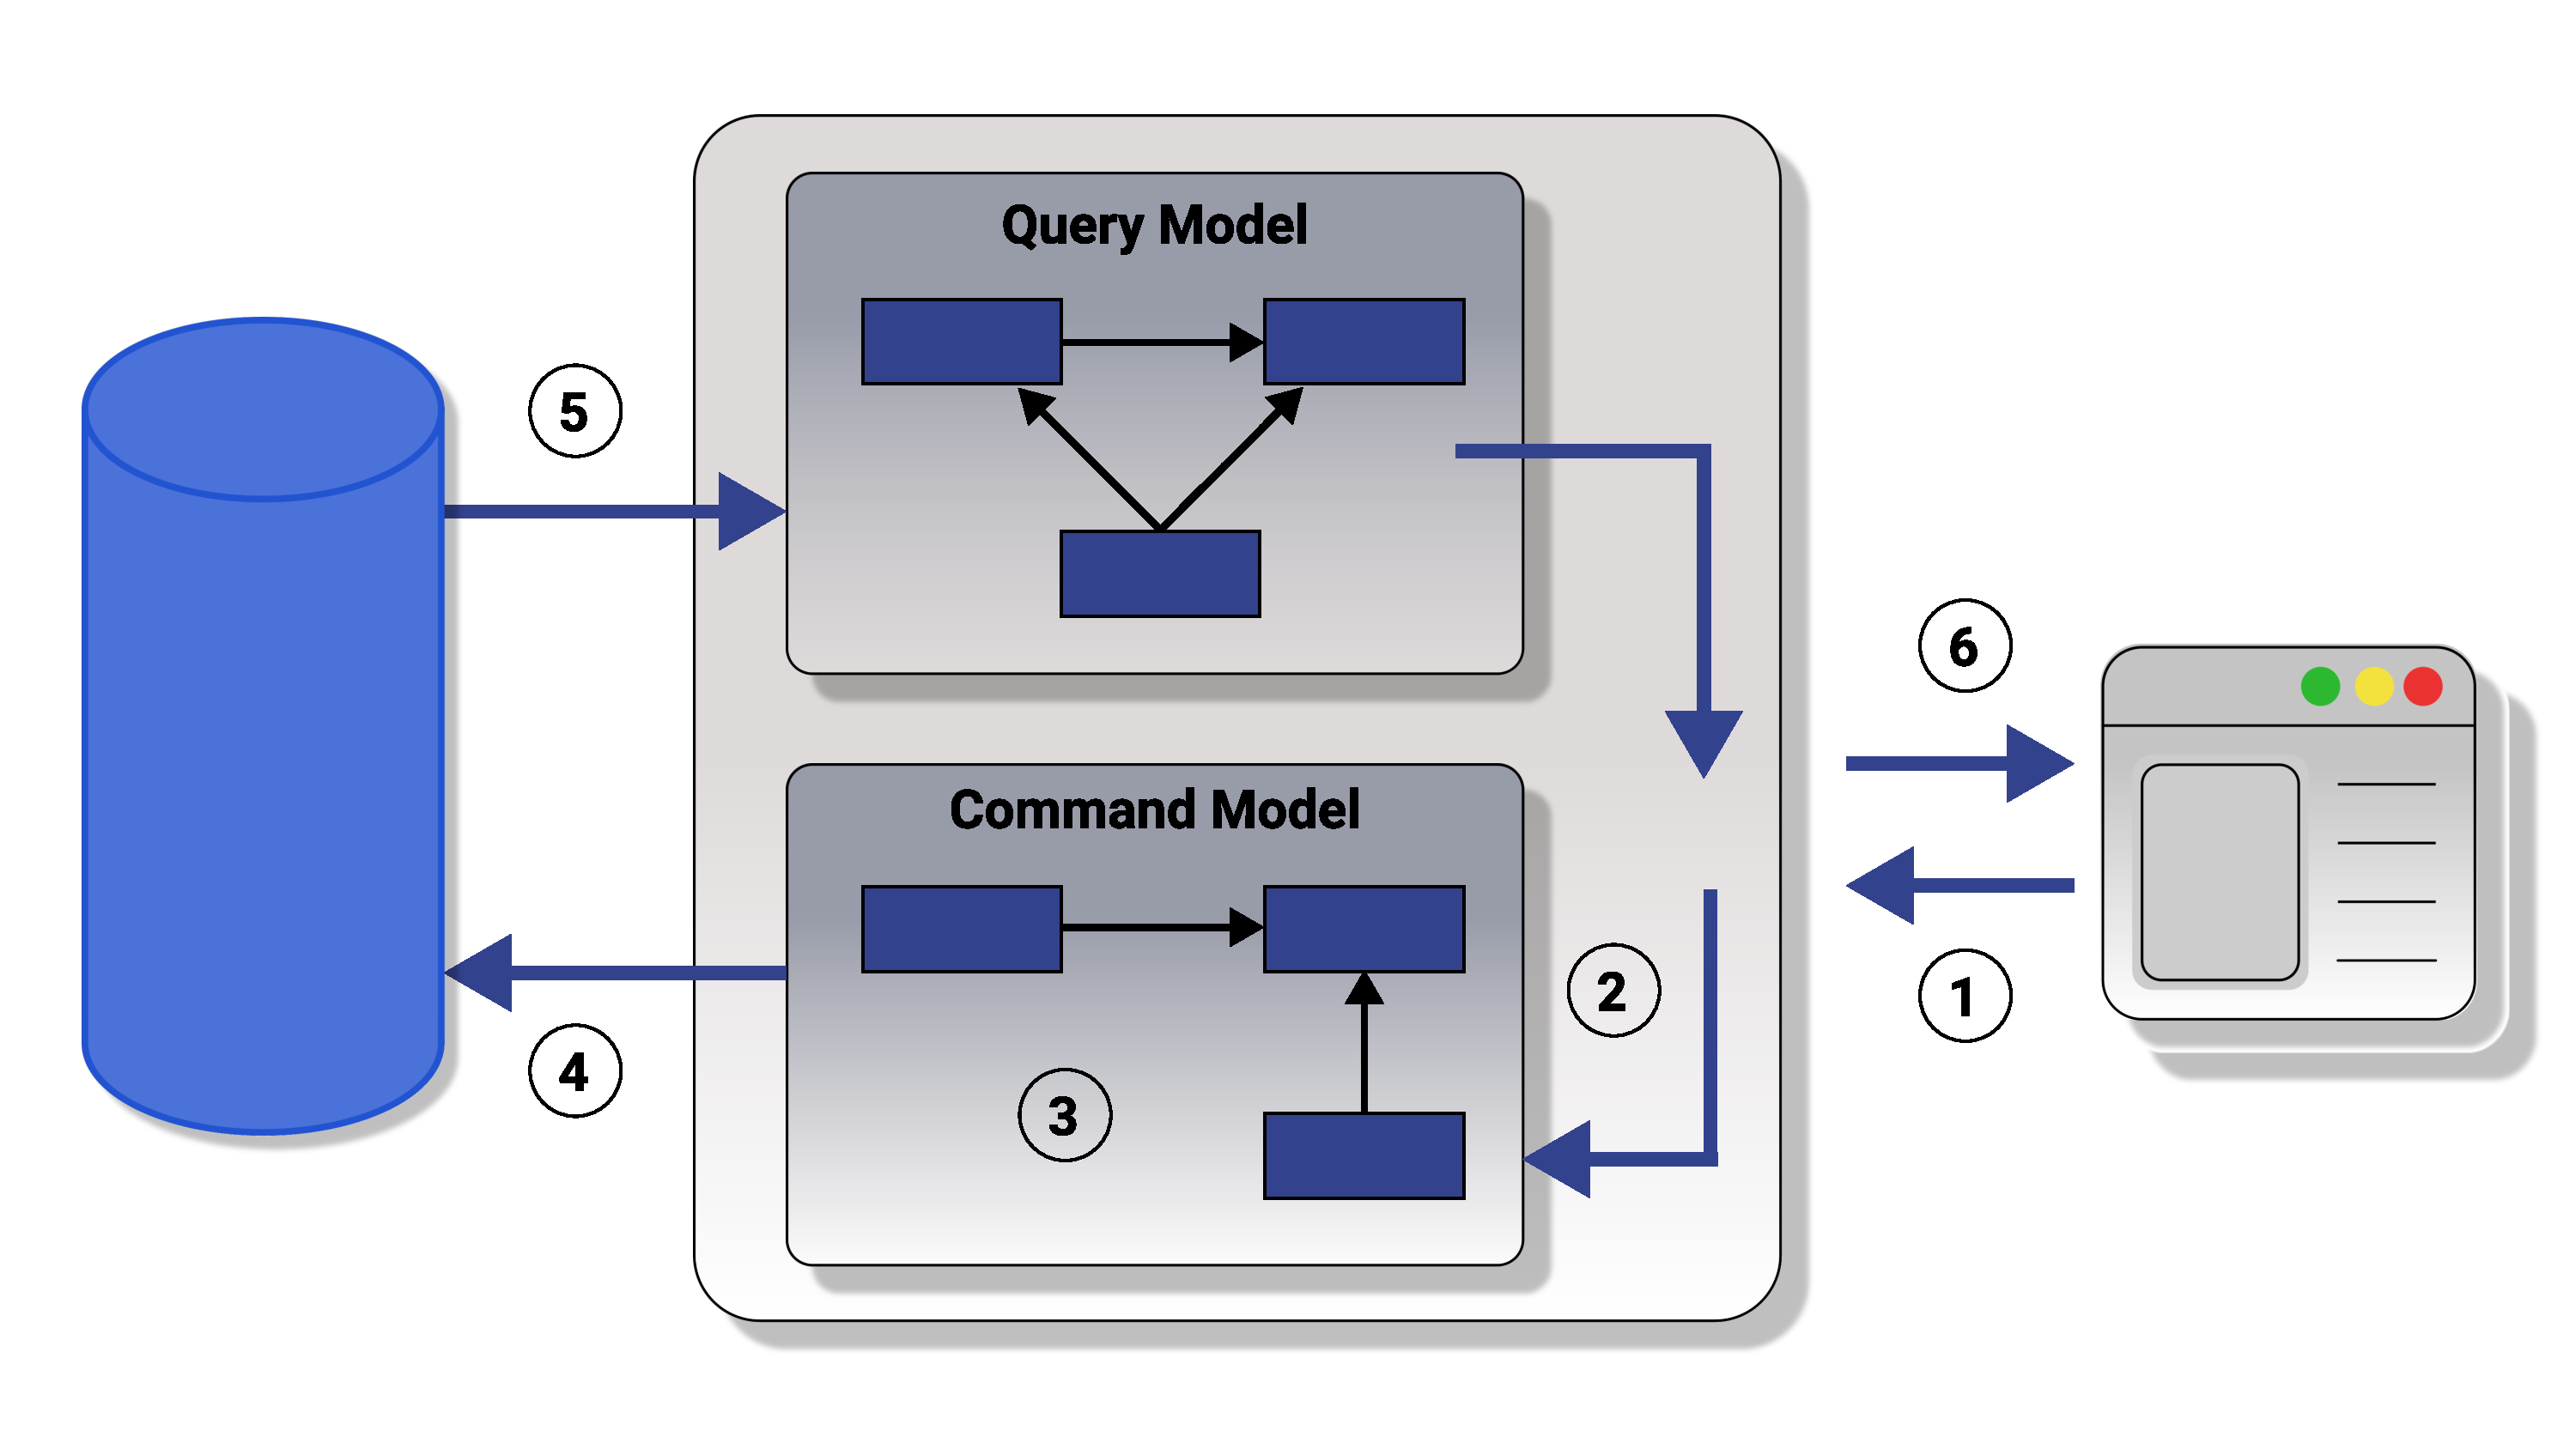
\includegraphics[width=1\textwidth]{Pictures/cqrs}
    \caption{CQRS Conceptual diagram. Source: https://martinfowler.com/bliki/CQRS.html}\label{fig:figure}
\end{figure}

\subsection{Discussion on JWT Authentication}\label{subsec:discussion-on-jwt-authentication}
\begin{figure}[H]
    \centering
    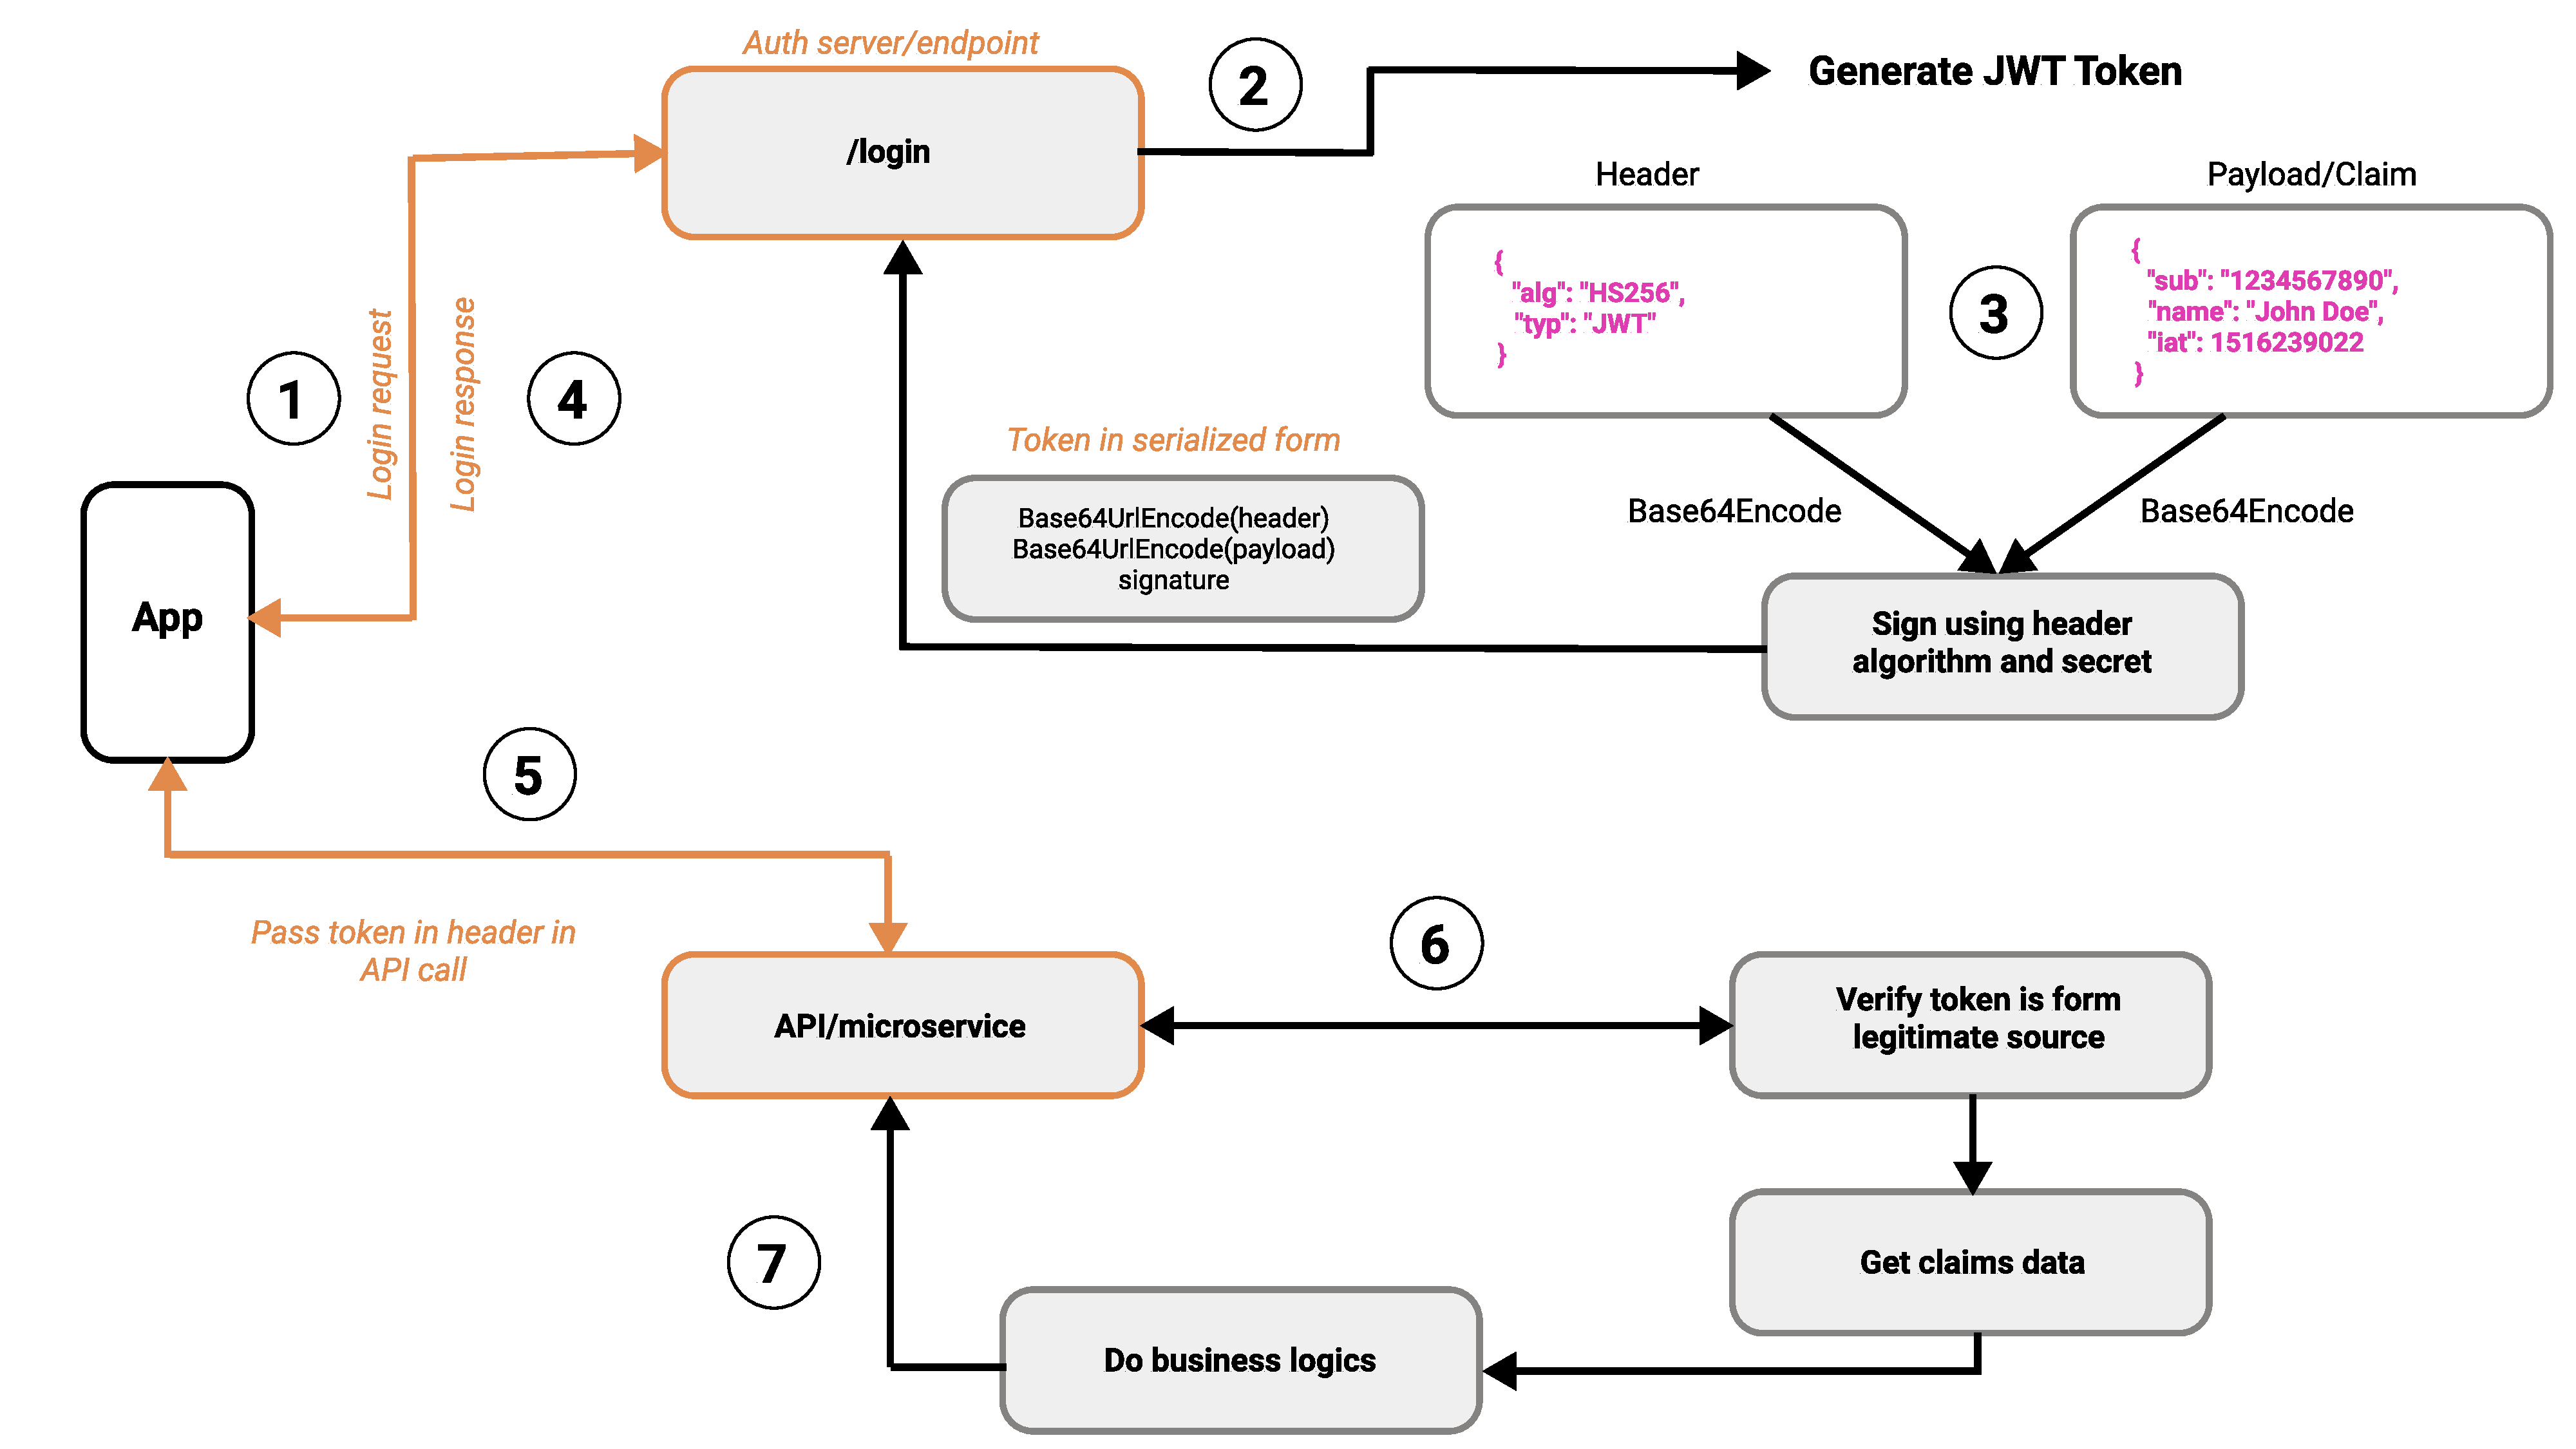
\includegraphics[width=1\textwidth]{Pictures/jwt_auth_scheme}
    \caption{CQRS Conceptual diagram. Source: https://martinfowler.com/bliki/CQRS.html}\label{fig:figure3}
\end{figure}

\subsection{Planned technologies}\label{subsec:planned-technologies}
Fill with technologies from readme file.


\section{Security aspects of HTTPS protocol}\label{sec:security-aspects-of-https-protocol}
General discussion on HTTP here.

\subsection{Diffie-Hellman Protocol}\label{subsec:diffie-hellman-protocol}
Diffie hellman protocol discussion here.